\chapter{The pgsynthdata Tool}
\label{ch:pgsynthdata_tool}
\section{Overview}
The tool is a single lightweight Python script, executable from the shell terminal. The tool first connects to an existing PostgreSQL database (based on the passed arguments) and then based on whether \mintinline{bash}{-show} or \mintinline{bash}{-generate} arguments were passed, with \mintinline{bash}{-show} being the default one. The tool also accepts database connection parameters (all optional) such as \mintinline{bash}{-H, -P, -U} for connecting to the desired database server.\\
The \mintinline{bash}{-show} argument (which is the default one) will show the configuration of the database and the \mintinline{bash}{-generate} argument generates the synthesized data to the database with the name \mintinline{bash}{DBNAMEGEN}, which is one of the required arguments for this tool.\\
To be continued...
\section{Design and Implementation}
This tool is written and coded using the Python programming language.\\
It uses various Python libraries that are used for: argument parsing, various mathematical functions, making the connection to the PostgreSQL server easier etc.\\
It is a single python script that is to be executed using the shell terminal. It requires some arguments/parameters initially in order to evaluate the PostgreSQL server it needs to connect to, what database it relies on for generating the synthetic data and also the database where the synthetic data will be generated on.\\
To be continued...
\subsection{Design Decisions}
\lipsum[2-3]
\section{Tool Usage}
The tool is very straightforward to use. It contains a single Python script, with all the logic of connecting to the database and showing/generating the data in a single script. It is a script, designed to be executed from the terminal shell using the python command.\\
The tool is somehow split into two parts. The first part is the database connection part, which, based on the arguments given for the database and the PostgreSQL connection parameters, tries to connect to that database instance in the server. If everything there is successful, the tool then continues with the data synthesis part.\\
\newline
\textbf{Tool usage:} \newline
\mintinline{bash}{pgsynthdata [OPTIONS]... DBNAMEIN [DBNAMEGEN]} \\
\newline
\textbf{Tool options:}
\begin{itemize}
\item \mintinline{bash}{DBNAMEGEN} - Name of the database to be created
\item \mintinline{bash}{-show/--show} - Shows config (default)
\item \mintinline{bash}{-generate/--generate} - Generates new synthesized data to database \textit{DBNAMEGEN}
\item \mintinline{bash}{-O/--owner} - Owner of new database (default: same as user)
\item \mintinline{bash}{-v/--version} - Show version information, then quit
\item \mintinline{bash}{-h/--help} - Show tool help, then quit
\newline
\end{itemize}
\textbf{Connection options:}
\begin{itemize}
\item \mintinline{bash}{DBNAMEIN} - Name of the existing database to connect to
\item \mintinline{bash}{-H/--hostname} - Name of the PostgreSQL server (default: \textit{localhost})
\item \mintinline{bash}{-P/--port} - Port of the PostgreSQL server (default: \textit{5432})
\item \mintinline{bash}{-U/--user} - PostgreSQL server username
\newline
\end{itemize}
\textbf{Some usage examples:}
\begin{itemize}
	\item \mintinline{bash}{python pgsynthdata.py test postgres -show}
	\begin{itemize}
		\item Connects to database \textit{test}, host=\textit{localhost}, port=\textit{5432}, default user with password \textit{postgres}
		\item Shows statistics from certain tables in database \textit{test}
	\end{itemize}
	\item \mintinline{bash}{python pgsynthdata.py db pw1234 -H myHost -p 8070 -U testuser -show}
	\begin{itemize}
		\item Connects to database \textit{db}, host=\textit{myHost}, port=\textit{8070}, user=\textit{testuser} with password \textit{pw1234}
		\item Shows statistics from certain tables in database \textit{db}
	\end{itemize}
	\item \mintinline{bash}{python pgsynthdata.py dbin dbgen pw1234 -H myHost -p 8070 -U testuser -generate}
	\begin{itemize}
		\item Connects to database \textit{dbin}, host=\textit{myHost}, port=\textit{8070}, user=\textit{testuser} with password \textit{pw1234}
		\item Creates new database \textit{dbgen} with synthesized data
	\end{itemize}
	\item \mintinline{bash}{python pgsynthdata.py --version}
	\begin{itemize}
		\item Show the version of this tool and then quit
	\end{itemize}
\end{itemize}
It also uses all the other default PostgreSQL server settings when creating the new database such as: encoding, locale, collation, database template etc.
\begin{figure}[H]
	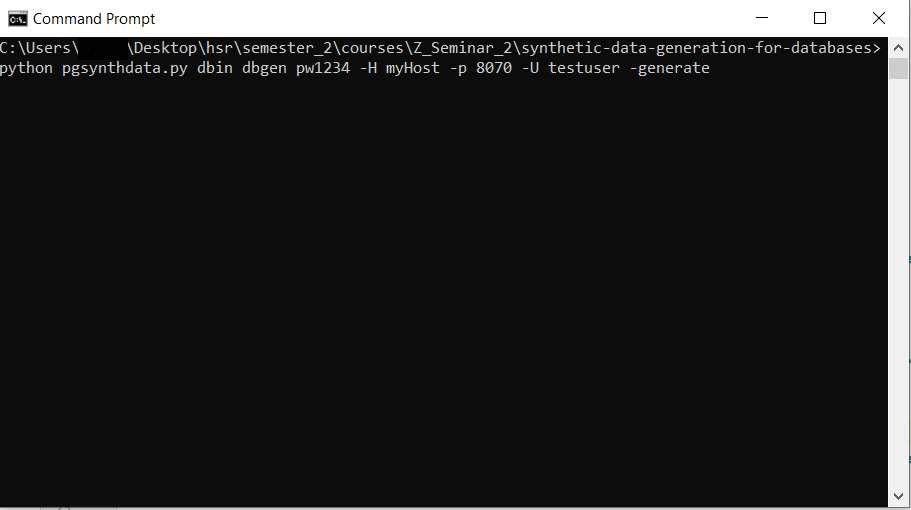
\includegraphics[width=\linewidth]{./Figures/Implementation/tool_example_cmd.png}
	\caption{Tool usage example}
\end{figure}